%----------------------------------------------------------------
%
%  File    :  survey-recc.tex
%
%  Author  :  Mirza Kabiljagic, Stefan Rajinovic, Aleksandar Stojicic,
%             Inti Gabriel Mendoza Estrada
%
%  Created :  27 May 20xx
%
%  Changed :  05 Dec 2019
%
%----------------------------------------------------------------

\chapter{Recommendation}
\label{chap:Recommendation}
 


\section{Recommendation}

Responsive tables must be able to efficiently and effectively display
data. It is only through a combination of good table design and
responsive techniques one is able to achieve this. 

For good table design, it is imperative that you include Alternate Row
Highlighting. This is a very simple technique that works on every
browser and is not only helpful to the user but to the developer as it
adds positively to the aesthetics. 

For a ``Jack of all trades'' approach, we suggest the following
responsive techniques: Long Two Column, and Fixed Header. You are able
to apply this for the 3 main screen sizes: PC, tablet, and phone.
Being able to apply Long Two Column to phone-sized screens (or tablets
in vertical mode) and leave Fixed Header on the remaining two sizes
(PC and tablets in horizontal mode) automatically eliminates one of
the 3 sizes you have to take care of. 

Another thing to keep in mind is to attach the vertical scrollable
feature of Fixed Header to the Long Two Column. This ensures that the
space the table is taking up is exactly the one allocated to it. It
goes without saying that if the table is too wide (horizontally), it
should be horizontally scrollable.

Figure \ref{fig:Recc1} shows these techniques working together. As you 
scroll through the table, notice the Fixed Header Technique in Figure 
\ref{fig:Recc2}. For small-sized screens, the technique that would ``kick 
in'' is shown in Figure \ref{fig:Recc3}. Notice the `creeping' second 
`minitable' in the bottom part.

\begin{figure}[tp]
    \centering
  
    {%
    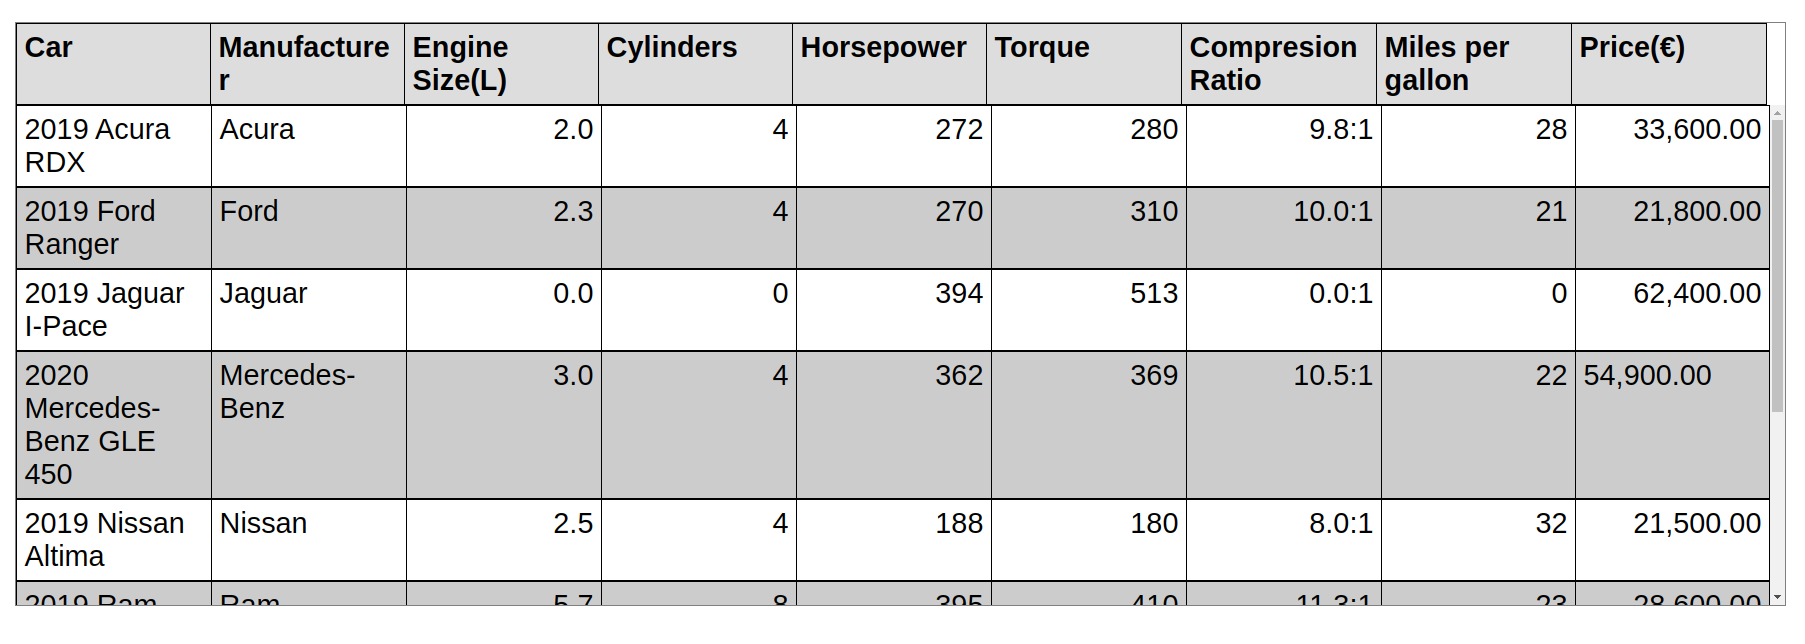
\includegraphics[width=1\linewidth]
    {images/recommendation_1.png}%
    \label{Recommendation 1}%
    }

    
    \caption[Recommendation Techniques 1]
    {
      
    \imgcredit{Screenshot taken by the author.}
    }
    \label{fig:Recc1}
\end{figure}



\begin{figure}[tp]
    \centering
  
    {%
    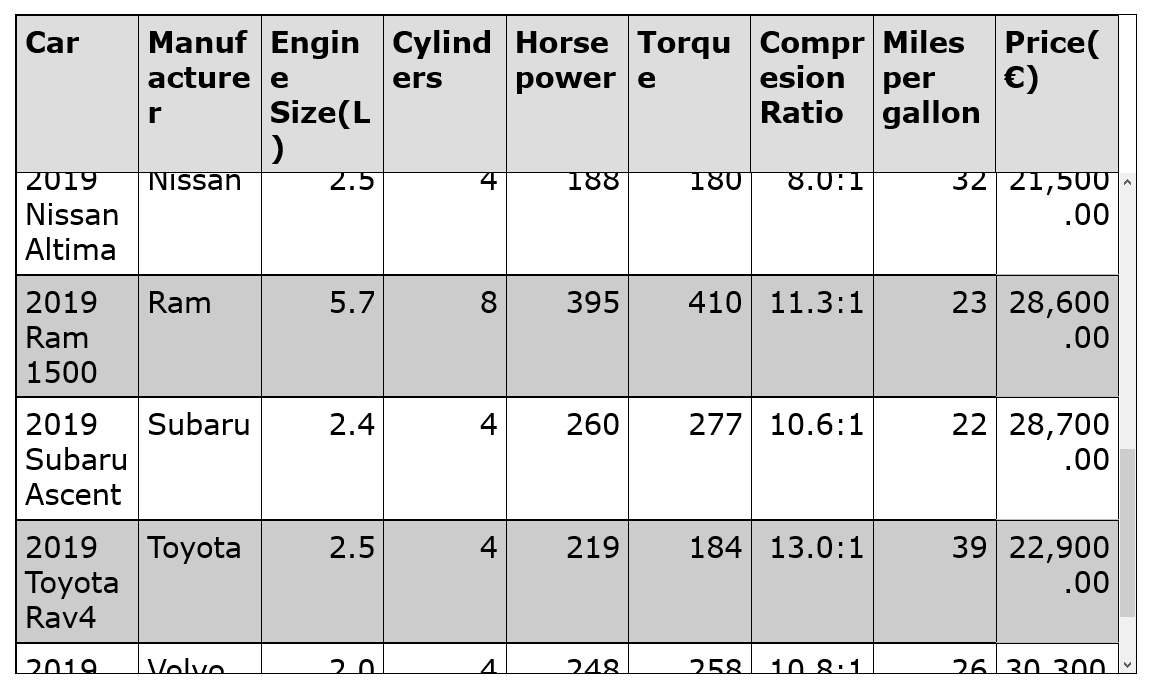
\includegraphics[width=0.75\linewidth]
    {images/recommendation_2.png}%
    \label{Recommendation 2}%
    }

    
    \caption[Recommendation Techniques 2]
    {
      
    \imgcredit{Screenshot taken by the author.}
    }
    \label{fig:Recc2}
\end{figure}



\begin{figure}[tp]
    \centering
  
    {%
    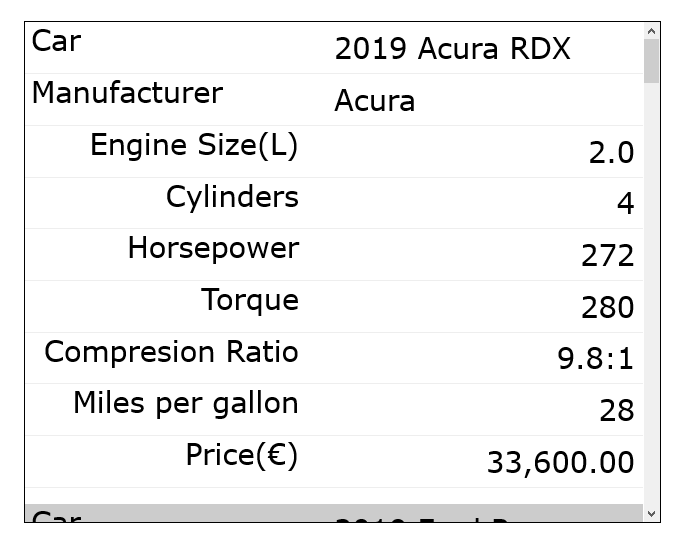
\includegraphics[width=0.5\linewidth]
    {images/recommendation_3.png}%
    \label{Recommendation 3}%
    }

    
    \caption[Recommendation Techniques 3]
    {
      
    \imgcredit{Screenshot taken by the author.}
    }
    \label{fig:Recc3}
\end{figure}



